
When training GAN models, the goal is to find a distribution $P_{\theta}$ that is the most similar to a real distribution $P_{r}$, with parameters $\theta$. One approach to acheiving this goal is to define a parametric family of densities $P_{\theta} \geq 0$, which is a differentiable. $P_{theta}$ can then be optimized through maximum likelihood estimation (MLE):

\begin{equation}
	\label{eq:mle}
	max_{\theta\in \mathbb{R}^{d}} \frac{1}{m} \sum_{i=1}^{m} log P_{\theta}(x^{(i)})
\end{equation}

Another way is to use a random variable $Z$ from a known distribution $p(z)$ and pass it through a tranformation function, $g_{\theta}$ to generate samples that from $P_{theta}$. This is what Generative Adverserial Networks do.

The second approach has two big advantages: it can represent distributions in a low dimension manifold, and unlike the densities, it is easier to generate samples of the distribution. In order to find a $P_{\theta}$ as close to $P_{r}$ as possible, the parameters $\theta$ needs to be optimized. 

To measure the similarity (distance) between the distributions, the authors introduce a new distance metric, the Earth Mover or Wasserstein-1 distance:

\begin{equation}
	\label{eq:em}
	W(P_{r}, P_{g}) = inf_{\gamma \in \Pi(P_{r},P_{g})} \mathbb{E}_{(x,y)~\gamma}[\Vert x - y \Vert]
\end{equation}

where $\Pi(P_{r}, P_{g})$ is the set of all joint distributions $\gamma(x,y)$ whose marginals are $P_{r}$ and $P_{g}$ and $\gamma$ intuitively represents the "mass" that must be moved from x to y in order to transform the distribution  $P_{g}$ into $P_{r}$. In other words, W is the "cost" of the optimal transport.

The Earth Mover distance (\ref{eq:em}) is preferable to \ref{eq:js} because it is defined even when both distribution are close to zero. 


\subsection{The WGAN}
The Earth Mover distance has many advantages, but one major problem is that its infimum is highly intractable. In order to use EM, Kantorovich-Rubinstein duality is used to approximate it:
\begin{center}
	$W(P_{r},P_{\theta}) = sup_{\Vert f \Vert_{L \leq 1}} \mathbb{E}_{x \sim P_{r}}[f(x)] - \mathbb{E}_{x \sim P_{\theta}}[f(x)] $
\end{center}
where the supremum is over all 1-Lipschitz functions f : X $\rightarrow$ R. Considering K-Lipschitz functions (instead of $f : \Vert f \Vert < 1, \Vert f \Vert < K$ ) for some constant K, then the supremum can be solved  for $K*W(P_{r}, P_{g})$, which is true because a K-Lipchitz function is a 1-Lipchitz function divided by K. Taking a parameterized family of  functions $f_{w}$, where w $\in$ W, w are the weights and W is the set of possible weights,  the supremum is still intractable, but can be approximated by:

\begin{center}
	$ max_{w \in W} \mathbb{E}_{x \sim P_{r}}[f_{w}(x)] - \mathbb{E}_{x \sim P_{\theta}}[f_{w}(x)] \leq sup_{\Vert f \Vert_{L \leq 1}} \mathbb{E}_{x \sim P_{r}}[f(x)] - \mathbb{E}_{x \sim P_{\theta}}[f(x)] = K * W(P_{r}, P_{\theta}) $
\end{center}

For optimization purposes, there is no need to know the value of K since it is a constant fixed throughout the process and will get absorbed into the hyperparameter tuning.


\subsubsection {Training}

Recall that the goal is for $P_{\theta}=P_{r}$. First, the optimal distance function $f_{w}$ is calculated for a fixed value $P_{\theta}$ of the generator. Then,  performing  backpropagation through $W(P_{r}, P_{\theta}(z))$ and sampling several z, the gradient for $\theta$ is found. The final step is to update $\theta$ and repeat the process. Figure \ref{fig:wgan} illustrates the process and the network's architecture. 

\begin{figure}[h!]
	\centering
	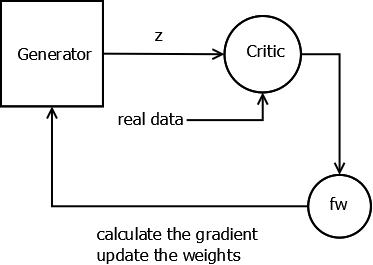
\includegraphics[scale=0.4]{media/WGAN.png}
	\caption{WGAN Architecture. Using $z$, the critic learns a function $f_w$ for estimating the distance between real and learned distributions.} 
	\label{fig:wgan}
\end{figure}

